% Hugh: my advice would be use \label{Is-Australia-at-risk-of-catching-rich-world-stagnation} in case you
% delete or reorder chapters. 
\chapter{How to avoid rich-world stagnation} \label{chap1} % \label{chap1} is used for cross-referencing - used \Cref{chap1} to refer to this chapter in the text  

This chapter sets out the per capita income experience of the rich world. It shows that 

\begin{itemize}
    \item in the long view income growth path across rich world has common factors / phases. Australia not that different. 
    \item in the mid view, there has been GFC divergence: rich world income growth weak Australian experience much better.
    \item shows that there is a risk of secular stagnation. spreading from ROW 
\end{itemize} 


\section{The long view: common experience of productivity growth including recent sustained slow PG}

Productivity growth around the rich world has followed a common pattern. It was fast postwar; slows down mid-70s, picks up for a bit 1990s, slow since early 2000s. Not much sign of productivity growth pickup. Aust not that different (\Cref{fig:mfp}).

Risk that low productivity will continue, but no way to tell. In any event, without TOT change, with workforce age share falling, Australia must push productivity growth and improve participation. \jim{Possible use of `don't count on high income growth' from budget pressures \& wealth of generations.}

\begin{figure}[p] 
 \caption{Long run averages of productivity growth in the rich world}
 \units{Average yearly percentage change in multi-factor productivity}
 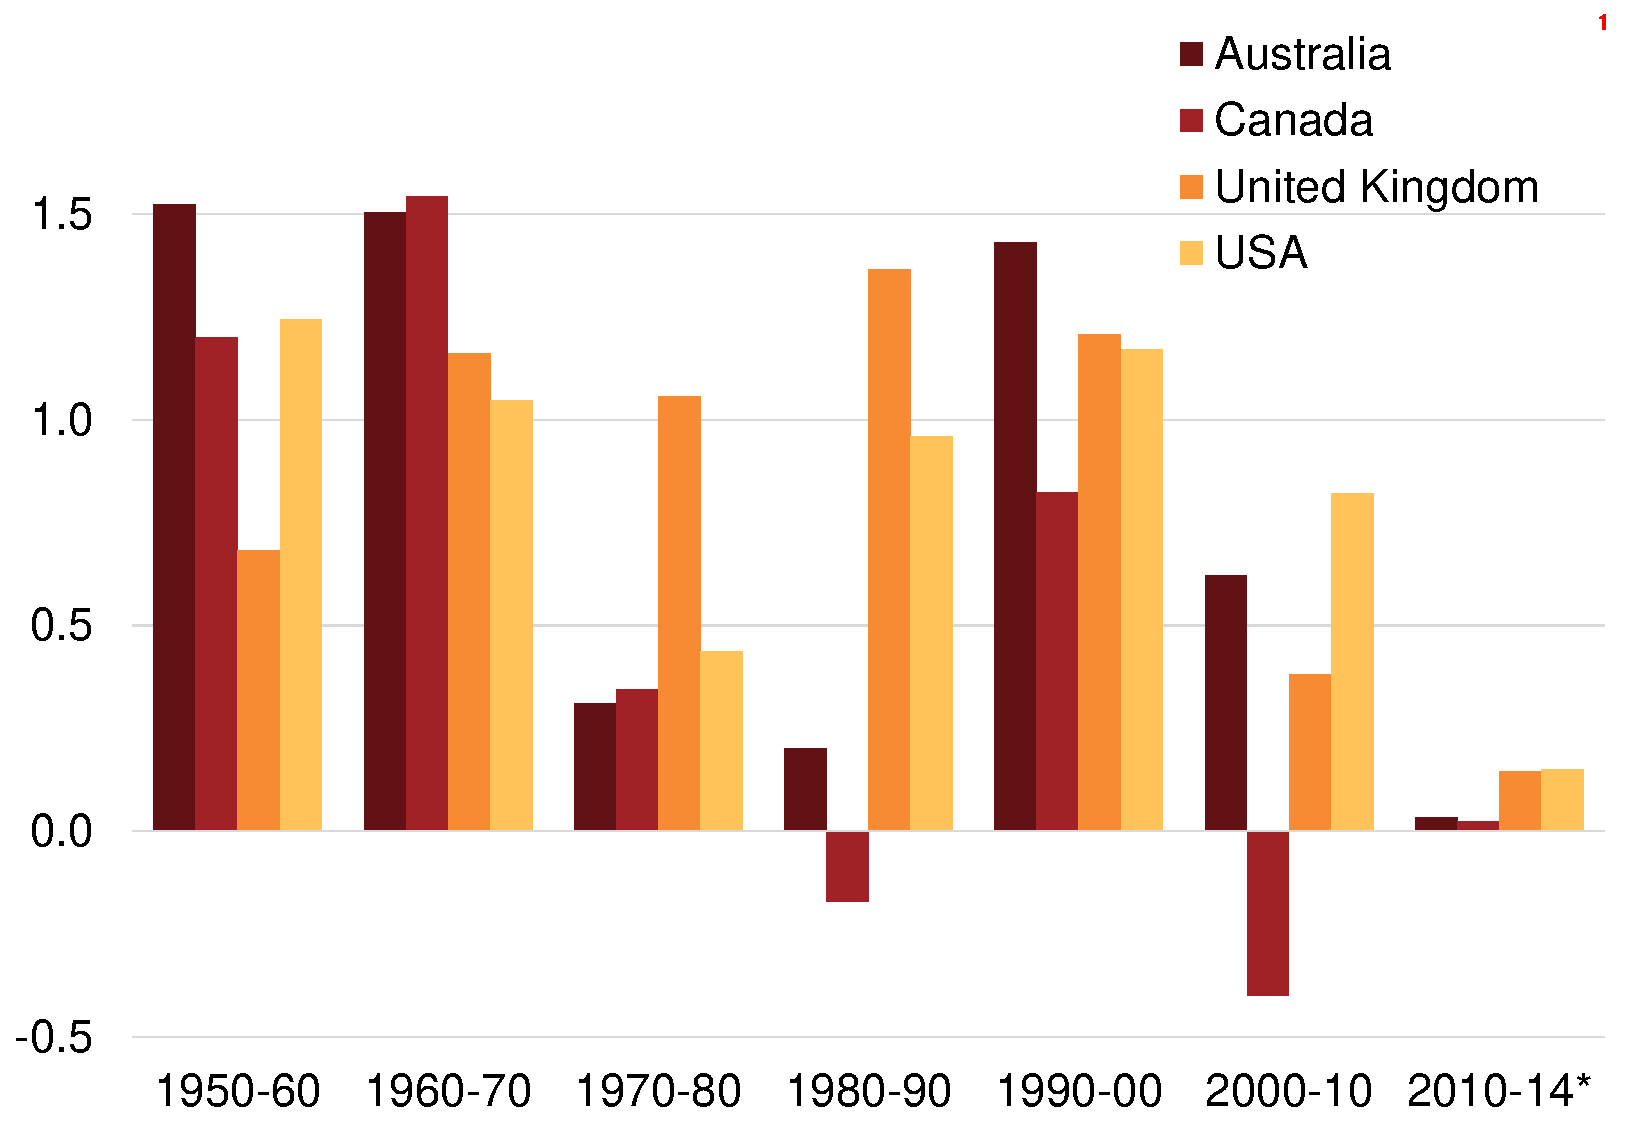
\includegraphics[page=1]{atlas/Ch1.pdf}\label{fig:mfp}
\notes{Bars for periods with US, Europe, Japan, Aust. Show that rich world had common factors. Could do income per capita first, much easier than MFP.}
\source{Penn World Tables v9.0, derived from TFP at constant national prices (2011=1) -- ***not consistent with Robert Gordon, confirm suitable data source***}
\end{figure}

\section{Mid-term: Until recently Australia has avoided the exceptionally weak post-GFC output growth}

Since the GFC, incomes have diverged. Rich world had a terrible time. Big fall in output in 09; Europe double dip; US steady but slow recovery; Australian experience much better (\Cref{fig:percap}).That is because the Australian financial system had limited exposure to toxic assets; demand was strong (policy; mining). While productivity growth was weak, strong input growth per capita meant good output growth per capita. And the TOT gave a massive boost to income til 2012.

And PS even Europe is starting to look better, though far below what had been expected. 

\begin{figure}[p] 
 \caption{Output per capita across the rich world since 2000}
  \units{GDP per capita, US Dollar (2010)}
 \includegraphics[page=2]{atlas/Ch1.pdf}\label{fig:percap}

\source{GDP per head, constant prices, constant exchange rates, OECD base year=2010, Units: US Dollar, 2010}

\notes{Just for Eurozone (not EU), US, Japan, Australia.} 
\jimi{Redo w PPPs}

\end{figure}

\section{There is some risk of `catching' secular stagnation}

8 years after the beginning of the global financial crisis, it now seems that rich economies can slip into long periods of 'secular stagnation' in which demand shortfalls and low capacity utilisation (of K, L) lead to low investment, with low 'natural' interest rates. 

There is some evidence \jim{or is it just theory at this stage} secular stagnation can spread across countries, depressed economies buy less from trade partners; if their central banks predominantly respond with low interest rates as main policy response (because part of the local expansion occurs via depreciation vs rest of world, which experiences an appreciation). Also add Caballero and \footcite{eggertsson2016} %\footcites{eggertsson2016}.

Commodity price channel?

Trading partner / asia / China risk.

Possibly Australia vulnerable to this. Mining investment comes off, but depreciation not as big as needed due to capital inflows. \jim{How true is this?} Example: when UK cut rates to a record low 0.25 per cent on August 4, and announced another GBP 60b of bond purchases, AUD rose X per cent vs ??

Secular stagnation is likely triggered by financial / macro, but can result in low productivity growth because firms invest less and may innovate less.

\section{To support growth, government needs `3 arrows'}

Not clear we need this section, but it could introduce the three areas.

\begin{itemize}
    \item keep investment going (mostly a macro issue; delicate balance of get back to sustainable budget position, monetary policy supportive)
    \item improve competitive intensity (micro; form of competition)
    \item work on spread of innovations (micro: ??)   
\end{itemize} 

See next chapters - 1 on each